\section{Advanced Specifications Implemented}\label{adv_mode_section}

\subsection{Problem Statement}
The objective of the \textit{ADVANCED} mode is to extend the behaviour of the baseline system so that the \gls{RGB} \gls{LED} reproduces, the colour measured by the \gls{RGB} sensor. Unlike the \textit{NORMAL} mode, where the \gls{LED} output follows predefined patterns, the \textit{ADVANCED} mode must directly map the sensor's \gls{RGB} data to the \gls{LED} output using the same relative chromatic composition.

Since the \gls{LED} pin assignment cannot be modified, the implementation must simulate \gls{PWM} in software in order to control the \gls{LED} brightness according to the sensor readings. All other functional parameters must remain identical to those of the \textit{NORMAL} mode.

\subsection{Implementation}
To reproduce the detected colour, the raw \gls{RGB} values obtained from the sensor are normalised with respect to the clear channel. This ensures that the emitted light preserves the chromatic ratios of the measured colour independently of the absolute illumination level.

A software-based \gls{PWM} mechanism is implemented to generate duty cycles proportional to the normalised \gls{RGB} components. The \gls{PWM} period is discretised into fixed-size steps, and during each step the \gls{LED} channels are switched on or off based on whether the current time index is below the computed duty threshold. This emulates real \gls{PWM} behaviour while keeping the original hardware configuration unchanged.

The following code fragment corresponds to the execution flow in \textit{ADVANCED} mode, after acquiring and displaying the colour measurements:

\begin{lstlisting}[language=C, caption={Software-based PWM implementation for ADVANCED mode}]
    #define PWM_STEP    1                          /**< PWM step in milliseconds. */
    #define PWM_PERIOD  15                         /**< PWM period in milliseconds. */
    #define PWM_STEPS   (PWM_PERIOD / PWM_STEP) /**< Number of PWM steps per period. */

    case ADVANCED_MODE:
        red(&leds);

        if(previous_mode != ADVANCED_MODE) {
            k_timer_stop(&rgb_timer);
            rgb_led_off(&rgb_leds);

            k_timer_stop(&main_timer);
            k_timer_start(&main_timer, K_MSEC(NORMAL_PERIOD), K_MSEC(NORMAL_PERIOD));
            previous_mode = ADVANCED_MODE;
        }

        k_sem_give(ctx.sensors_sem);
        k_sem_give(ctx.gps_sem);

        k_sem_take(ctx.main_sensors_sem, K_FOREVER);
        k_sem_take(ctx.main_gps_sem, K_FOREVER);

        get_measurements();

        display_measurements();

        if (main_data.c <= 0.0f) {
            printk("[WARN] - Color clear channel == 0\n");
            r_norm = g_norm = b_norm = 0.0f;
        } else {
            r_norm = (main_data.r / main_data.c) * 100.0f;
            g_norm = (main_data.g / main_data.c) * 100.0f;
            b_norm = (main_data.b / main_data.c) * 100.0f;
        }
        
        printk("NORMALIZED COLOR VALUES: R: %.2f%%, G: %.2f%%, B: %.2f%%\n\n",
                (double)r_norm, (double)g_norm, (double)b_norm);
        
        r_duty = (int)(r_norm * PWM_STEPS / 100);
        g_duty = (int)(g_norm * PWM_STEPS / 100);
        b_duty = (int)(b_norm * PWM_STEPS / 100);
        
        keep_running = true;
        while (keep_running) {
            for (int t = 0; t < PWM_PERIOD; t += PWM_STEP) {
                r_value = (t < r_duty) ? 1 : 0;
                g_value = (t < g_duty) ? 1 : 0;
                b_value = (t < b_duty) ? 1 : 0;
        
                rgb_led_pwm_step(&rgb_leds, r_value, g_value, b_value);
                k_sleep(K_MSEC(PWM_STEP));
        
                if (k_sem_take(&main_sem, K_NO_WAIT) == 0) {
                    keep_running = false;
                    break;
                }
            }
        }
\end{lstlisting}

During development, several timing constraints were encountered when attempting to reduce the \gls{PWM} step below the millisecond scale. The Zephyr scheduler, together with the hardware capabilities of the target board, prevented reliable delays shorter than one millisecond when using \texttt{k\_sleep()}. 

Alternative approaches were evaluated, including the use of \texttt{k\_busy\_wait()} to achieve microsecond-level blocking delays. However, the board exhibited unstable behaviour and noticeable performance degradation when executing busy-wait loops within the real-time colour reproduction cycle. Consequently, the software \gls{PWM} design was constrained to millisecond-resolution timing.

\subsubsection{Macro definitions and timing parameters}
\label{sssec:macros}
\begin{lstlisting}[language=C, caption={Macros for \textit{ADVANCED} mode}]
#define PWM_STEP    1                          /**< PWM step in milliseconds. */
#define PWM_PERIOD  15                         /**< PWM period in milliseconds. */
#define PWM_STEPS   (PWM_PERIOD / PWM_STEP) /**< Number of PWM steps per period. */
\end{lstlisting}

These macros define the temporal discretisation used by the software PWM:

\begin{itemize}
  \item \texttt{PWM\_STEP} specifies the length of a single PWM step in milliseconds. Each step is one atomic time-slot in which the LED channels are either ON or OFF.
  \item \texttt{PWM\_PERIOD} is the total duration of one PWM cycle in milliseconds. The perceived brightness is determined by the fraction of this period during which a channel is ON.
  \item \texttt{PWM\_STEPS} is the number of discrete steps per PWM period (computed as \texttt{PWM\_PERIOD / PWM\_STEP}). It is used to convert percentage-based normalised colour values into integer duty counts.
\end{itemize}

This configuration intentionally uses millisecond resolution due to the underlying RTOS scheduler and board timing limitations discussed previously.

\subsubsection{Sensor clear-channel safety check and normalisation}
\label{sssec:normalisation}
\begin{lstlisting}[language=C, caption={Color normalisation based on clear channel}]
if (main_data.c <= 0.0f) {
    printk("[WARN] - Color clear channel == 0\n");
    r_norm = g_norm = b_norm = 0.0f;
} else {
    r_norm = (main_data.r / main_data.c) * 100.0f;
    g_norm = (main_data.g / main_data.c) * 100.0f;
    b_norm = (main_data.b / main_data.c) * 100.0f;
}
\end{lstlisting}

Explanation:
\begin{itemize}
  \item \texttt{main\_data.c} denotes the clear (ambient) channel returned by the colour sensor. A zero or negative value indicates an invalid or saturated measurement.
  \item The \textbf{safety check} prevents division by zero by forcing the normalised channels to 0\% and emitting a warning via \texttt{printk} if the clear channel is non-positive.
  \item When valid, each raw channel (\texttt{r}, \texttt{g}, \texttt{b}) is normalised by the clear channel and converted to percentage units by multiplying by 100. This preserves the chromatic ratios while removing absolute intensity dependence.
\end{itemize}

\subsubsection{Diagnostic logging}
\label{sssec:logging}
\begin{lstlisting}[language=C, caption={Diagnostic logging of normalised color values}]
printk("NORMALIZED COLOR VALUES: R: %.2f%%, G: %.2f%%, B: %.2f%%\n\n",
        (double)r_norm, (double)g_norm, (double)b_norm);
\end{lstlisting}

Explanation:
\begin{itemize}
  \item This log statement prints the computed normalised percentages for each channel. It serves as a diagnostic aid during development and in-field debugging to verify that sensor readings and normalisation behave as expected.
  \item Casting to \texttt{double} is used to satisfy the \texttt{printk} format specifier and to ensure consistent formatting across platforms.
\end{itemize}

\subsubsection{Duty-cycle computation}
\label{sssec:duty}
\begin{lstlisting}[language=C, caption={Computation of duty counts from normalised percentages}]
r_duty = (int)(r_norm * PWM_STEPS / 100);
g_duty = (int)(g_norm * PWM_STEPS / 100);
b_duty = (int)(b_norm * PWM_STEPS / 100);
\end{lstlisting}

Explanation:
\begin{itemize}
  \item The normalised percentages are converted into integer \emph{duty counts} that range from 0 to \texttt{PWM\_STEPS}.
  \item Example: with \texttt{PWM\_STEPS = 15}, a normalised red value of 50\% results in \texttt{r\_duty = 7} (approximately half of the period steps ON).
  \item Integer truncation is acceptable here because the PWM resolution is limited by \texttt{PWM\_STEPS}; if higher fidelity is required, increase \texttt{PWM\_STEPS} by reducing \texttt{PWM\_STEP}, subject to the timing limits of the platform.
\end{itemize}

\subsubsection{Main PWM loop and per-step evaluation}
\label{sssec:mainloop}
\begin{lstlisting}[language=C, caption={Main software PWM loop}]
keep_running = true;
while (keep_running) {
    for (int t = 0; t < PWM_PERIOD; t += PWM_STEP) {
        r_value = (t < r_duty) ? 1 : 0;
        g_value = (t < g_duty) ? 1 : 0;
        b_value = (t < b_duty) ? 1 : 0;

        rgb_led_pwm_step(&rgb_leds, r_value, g_value, b_value);
        k_sleep(K_MSEC(PWM_STEP));

        if (k_sem_take(&main_sem, K_NO_WAIT) == 0) {
            keep_running = false;
            break;
        }
    }
}
\end{lstlisting}

Step-by-step explanation:
\begin{enumerate}
  \item \texttt{keep\_running} controls the outer loop that maintains continuous PWM operation until an external condition requests termination.
  \item The inner \texttt{for} loop iterates over the PWM period in increments of \texttt{PWM\_STEP}. The loop variable \texttt{t} effectively indexes the current step within the period.
  \item For each step, the boolean channel values (\texttt{r\_value}, \texttt{g\_value}, \texttt{b\_value}) are computed by comparing the current step index \texttt{t} with the corresponding duty count. If the index is strictly less than the duty count, the channel is considered ON for that step.
  \item \texttt{rgb\_led\_pwm\_step(...)} is the hardware abstraction that applies the computed ON/OFF values to the LED pins. It is expected to be non-blocking and to update GPIO (or LED driver) outputs accordingly.
  \item \texttt{k\_sleep(K\_MSEC(PWM\_STEP))} yields the CPU for the duration of one step. This implements the time base for the PWM emulation while allowing other RTOS threads to run.
    \item After sleeping, the loop checks \texttt{k\_sem\_take(\&main\_sem, K\_NO\_WAIT)} to determine whether a semaphore has been signalled. If the semaphore is available, the loop exits gracefully. The semaphore is triggered either when the user presses the button or when the 30-second timeout associated with each \textit{ADVANCED} mode cycle elapses.
\end{enumerate}

\subsection{Result}\label{adv_results}

The software-based \gls{PWM} strategy successfully reproduces the colour detected by the \gls{RGB} sensor. The \gls{LED} output maintains the chromatic proportions observed in the ambient light, while ensuring smooth transitions and stable operation. The colour is not exact since the \gls{PWM} resolution is limited to 1 ms steps and the light reflection on the measured object affects the perceived colour, but the representation is sufficiently precise for visual indication applications.

\begin{figure}[H]
    \centering
    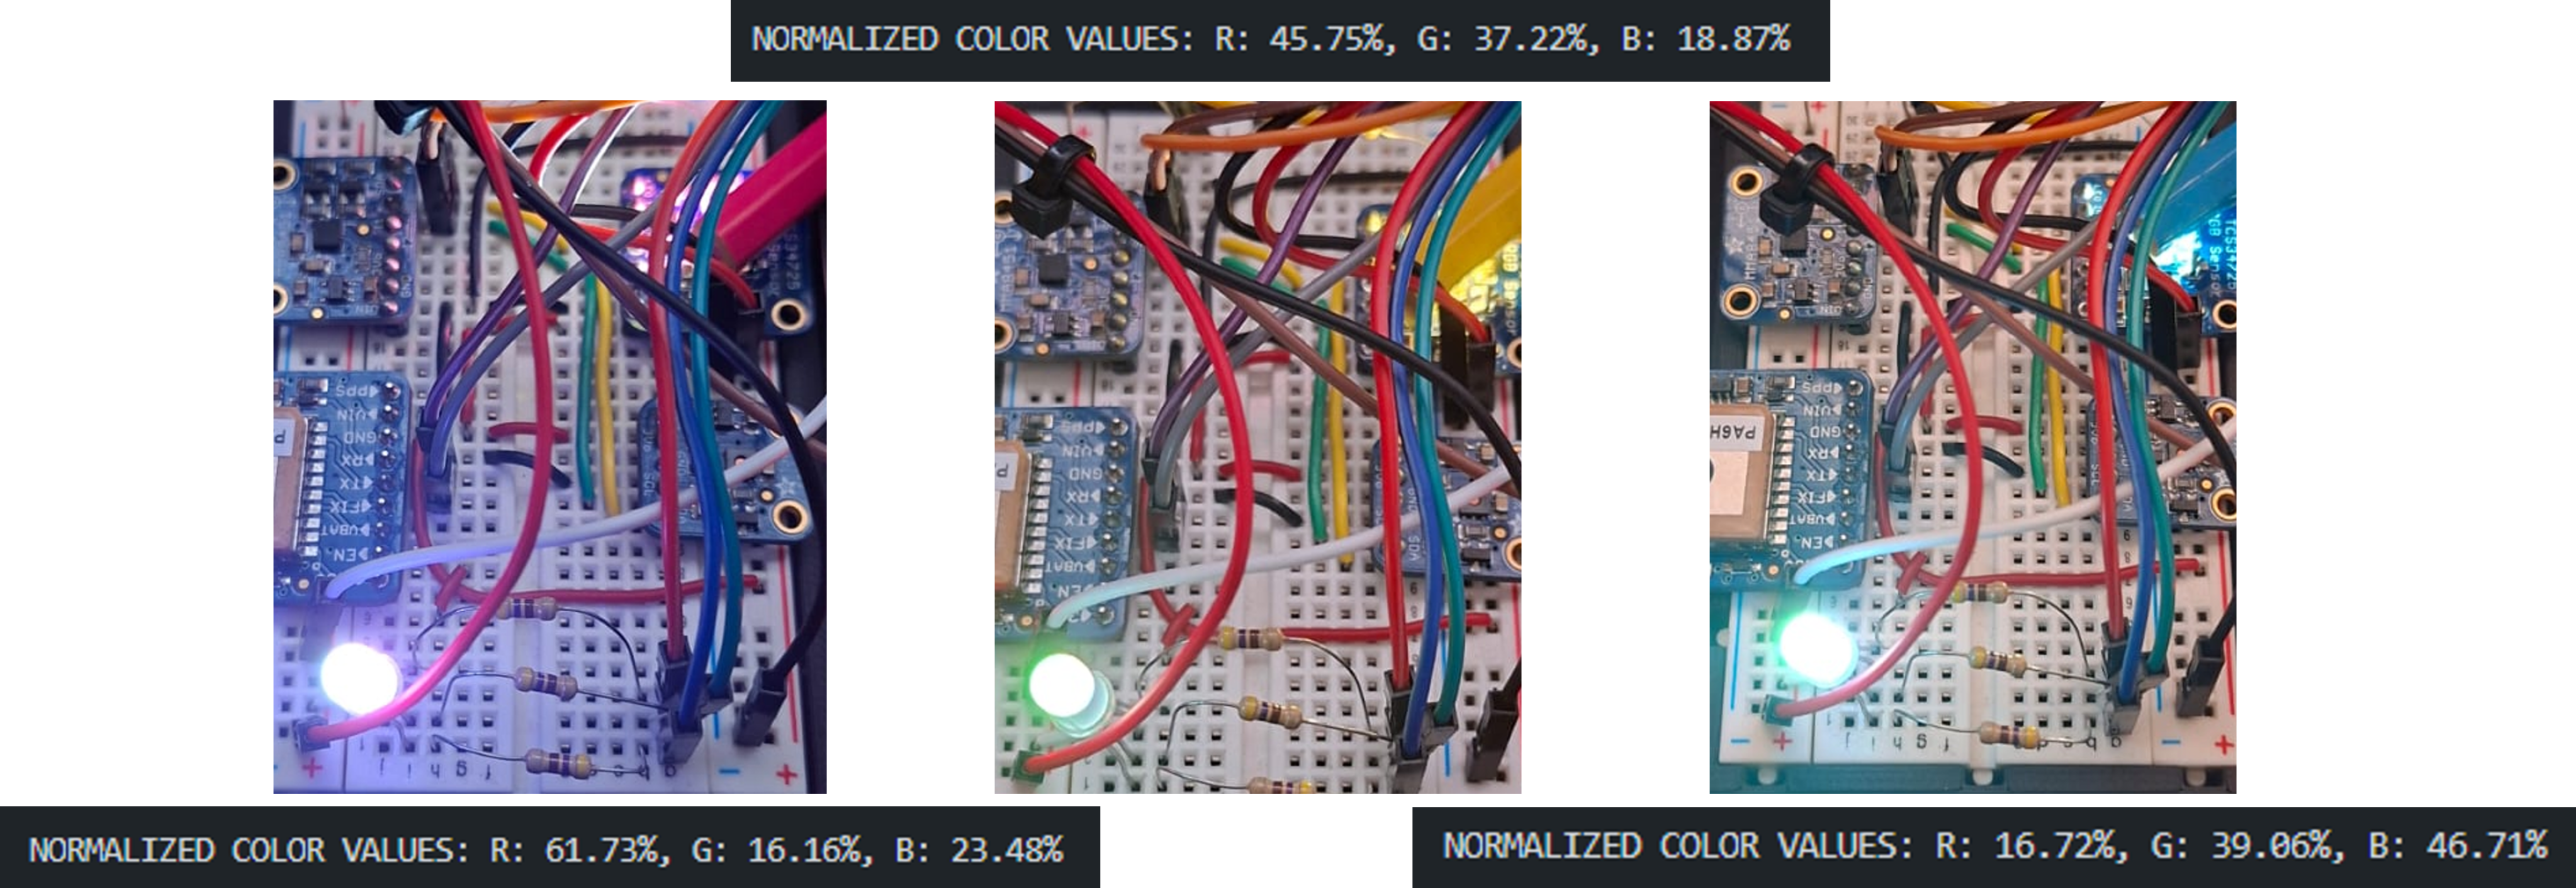
\includegraphics[width=0.99\textwidth]{images/pwm_res.png}
    \caption{\acrshort{PWM} emulated for \textit{ADVANCED} mode}
    \label{fig:pwm_res}
\end{figure}

The system preserves full compatibility with the existing hardware configuration and maintains identical behaviour to the \textit{NORMAL} mode regarding synchronisation, timing, and user interaction.

